%% Document class
\documentclass[final,3p,times,twocolumn, 12pt]{elsarticle}
% two column format
% \documentclass[preprint,review,12pt]{elsarticle}        % one column format

%% Use package
\usepackage{graphicx}
%\usepackage{epstopdf}
\usepackage{amssymb}
\usepackage{amsthm}
\usepackage{amsmath}
\usepackage{latexsym}
\usepackage{mathrsfs}
\usepackage[tight,nice]{units}
\usepackage{harpoon}
\usepackage{chemarrow}
\usepackage{lineno}
\usepackage{harpoon}
\usepackage{chemarrow}
\usepackage{lscape}
\usepackage{color}
\usepackage{lineno}
\usepackage{colortbl}
\usepackage{chngcntr}
% \usepackage{etoolbin}
\usepackage{tikz}
\usepackage{enumitem}
\usepackage{float}
\usepackage{soul}
\usepackage{url}
\usepackage{xr}
\usepackage{nomencl}
\usepackage{xstring}
\usepackage{xpatch}
\usepackage{bm}
\usepackage{lineno}
\linenumbers

\usepackage[hidelinks]{hyperref}
\biboptions{super,sort&compress}
\usepackage{orcidlink}
\newcommand{\bluelink}[2]{%
  \href{#1}{\textcolor{blue}{#2}}%
}
% Figure sizes
% Full textwidth for this template is ~ 6.47in
% A single column width for the template is ~ 3.07in

%% Change margins
\geometry{top=1in, bottom=1in}

%% Add line numbers
% \linenumbers

%% Submittal Material - Moves all figures to end of document
% \usepackage{endfloat}

%% Bib options
% \biboptions{sort&compress}%,super}

%% Cross referencing option
\makeatletter
\newcommand*{\addFileDependency}[1]{
    \typeout{(#1)}
    \@addtofilelist{#1}
    \IfFileExists{#1}{}{\typeout{No file #1.}}  }

\makeatother
\newcommand*{\myexternaldocument}[1]{
    \externaldocument{#1} 
    \addFileDependency{#1.tex} 
    \addFileDependency{#1.aux}  }
    
\myexternaldocument{supplementary}

%% Eliminates automatic footer note
\makeatletter
\def\ps@pprintTitle{%
  \let\@oddhead\@empty
  \let\@evenhead\@empty
  \let\@oddfoot\@empty
  \let\@evenfoot\@oddfoot  }

%% New commands
\newcommand{\crr}[1]{\color{red} #1 \color{black}}
\newcommand{\scd}[1]{\color{red} #1 \color{black}} % red field for edits

%% Nomenclature - changed name, set groups
% In the future, build this throughout the document because sorting is done automatically.
% Just remember to put header letter followed by sorting name in optional argument.
%   For an example, see end of the document.
\renewcommand{\nomlabelwidth}{1.25cm}
\setlength{\nomitemsep}{-\parsep}

% \renewcommand{\nomname}{List of Symbols}

% \patchcmd{\thenomenclature}
%   {\leftmargin\nomlabelwidth}
%   {\leftmargin\nomlabelwidth}
%   {}{}

% \newcommand{\nomenclheader}[1]{%
%   \item[\hspace*{-\itemindent}\normalfont\bfseries#1]}
% \renewcommand\nomgroup[1]{%
%   \IfStrEqCase{#1}{%
%    {A}{\nomenclheader{Roman Symbols}}%                  
%    {B}{\\ \nomenclheader{Greek Symbols}}%                 
%    {C}{\\ \nomenclheader{Subscripts and Superscripts}}%    
%   }%
% }
  
% \makenomenclature

\newpageafter{author}

%% Begin document
\begin{document}

\begin{frontmatter}

\title{Particle Tracking Methods for Battery Precipitation Reactions}

\author[CSM]{Trent Koberna}
\author[CSM]{Steven C. DeCaluwe \corref{cor}}
\cortext[cor]{Corresponding Author: Tel: (303) 273-3666}
\ead{decaluwe@mines.edu}
        
\address[CSM]{Colorado School of Mines Department of Mechanical Engineering, 1500 Illinois St, Golden, CO 80401}

%%%%%%%%%%%%%%%%%%%%%%%%%%%%%%%%%%%%%%%%%%%%%%%%%%%%%%%%%%%%%%%%%%%%%%%%%%


\end{frontmatter}
\onecolumn
\noindent Precipitation and deposition reactions at solid-liquid interfaces play a key role in a number of battery chemistries, including Li-ion, so-called `anode free' batteries, zinc-based battery chemistries, and lithium-sulfur, among others. Although models with heterogeneous nucleation and growth phenomena are present in the literature, papers have not to date provided much detail on the numerical algorithms used to track the temporal evolution of the particle size distribution of deposits on electrode surfaces.  In this letter we examine several approaches to discretize and track the particle size distribution, demonstrating that common approaches lead to anomalous `flattening' of the particle size distribution.  We conclude by presenting an algorithm that preserves the appropriate particle size distribution during particle growth.\\ 
\\ 
\noindent \textit{Keywords:} Heterogeneous Nucleation and Growth, Deposition reactions, Batteries\\
\\ 
\noindent TOC Graphic
\begin{center}
    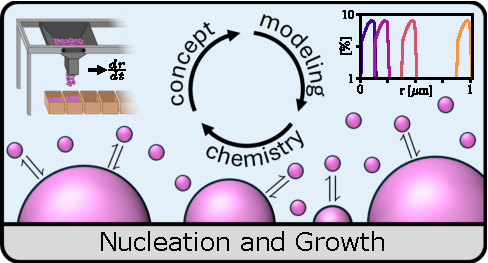
\includegraphics[scale=1]{figures/TOC.pdf}
\end{center}





\newpage
%%%%%%%%%%%%%%%%%%%%%%%%%%%%%%%%%%%%%%%%%%%%%%%%%%%%%%%%%%%%%%%%%%%%%%%%

\section{Introduction}
Precipitation and deposition reactions play key roles in a number of battery applications, including both intercalation-type Li-ion  and ``beyond Li-ion'' batteries. Specific examples include:
    \begin{itemize}
        \item \textit{Bulk solid storage}: During charging in so-called `anode-free' batteries, Li metal deposits nucleate and then grow on a bare copper current collector~\cite{bib:Li-Cu_deposition}. The nucleation and growth dynamics significantly impact the Li morphology, which directly controls device durability. \cite{bib:PSD_effects_Li,bib:PSD_effects_Li_2,bib:PSD_effects_Li_3,bib:PSD_effects_Li_4,bib:Model_ex_1}
        
        \item \textit{Interfacial growth}: In batteries such as lithium-sulfur and lithium-oxygen, dissolved liquid electrolyte species are reduced during discharge, depositing and growing on the cathode surface. The capacity and rate capability are sensitive to the precipitate nucleation density~\cite{bib:Li-S_deposition,bib:Li-S_deposition_2,bib:Li-O_deposition,bib:Li-air_deposition,bib:Model_ex_2,bib:Model_ex_8}.
               
        \item \textit{SEI formation}: The solid electrolyte interphase (SEI) is a multi-phase passivation layer on the anode surface, formed via deposition of insoluble electrolyte degradation products. The number, size, and distribution of individual phases determine the layer's ionic conductivity and long-term stability and are controlled by nucleation and growth phenomena~\cite{bib:SEI_deposition,bib:SEI_deposition_2,bib:SEI_deposition_3}.
    \end{itemize}

Such deposition reactions typically proceed through two steps.~\cite{bib:classic_nuc_theory} New precipitates first nucleate at the liquid-solid interface. This creates new material interfaces (precipitate-substrate and precipitate-liquid), and therefore includes a significant energy barrier\cite{bib:Model_ex_2}. As such, nucleation typically requires supersaturation of the liquid solution, with the nucleation rate (and thus the number of deposited nuclei) increasing with the degree of supersaturation\cite{bib:supersat}.  After nucleation, growth proceeds with a rate that is proportional to the number of nuclei deposited. Because the growth energy barrier is lower than that for nucleation, the degree of supersaturation typically decreases  during growth, such that nucleation rates are typically low during the growth phase\cite{bib:Li-Cu_deposition}.

Correctly modeling precipitate deposition and  growth is critical to predicting device performance and degradation for efficient and durable devices. Numerous studies have incorporated heterogeneous nucleation and growth (HNG) kinetics into device simulations.~\cite{bib:Model_ex_1,bib:Model_ex_2,bib:Model_ex_3,bib:Model_ex_4,bib:Model_ex_5,bib:Model_ex_6, bib:Model_ex_7, bib:Model_ex_8,bib:Model_ex_9, bib:Model_ex_10} However, there is less detail in the literature describing the method by which these models track the particle size distribution (PSD) of surface precipitates in these systems. This letter evaluates some common approaches to PSD tracking and proposes an algorithm to properly track the PSD during HNG, using a simplified kinetic mechanism to clearly evaluate the PSD accuracy. 

%%%%%%%%%%%%%%%%%%%%%%%%%%%%%%%%%%%%%%%%%%%%%%%%%%%%%%%%%%%%%%%%%%%%%%%%%%
\section{Model framework}
\label{sect:model-framework}
\subsection{Kinetic Model Assumptions}
For easy-to-interpret results, we use a relatively simple kinetic model:
\begin{itemize}
    \item \emph{Nucleation phase}: Hemispherical nuclei with radius $r_{\rm nuc}=0.5$~nm are deposited at a rate $\dot{q}_\mathrm{nuc}''$ from $t = 0$~s to $t = 0.5$~s.
    \item \emph{Particle growth}: Once a particle is formed, it grows at a constant rate of $\frac{dr}{dt} = 0.25~\mu$m s$^{-1}$.
\end{itemize}
This growth rate is equivalent to a deposition rate of $\dot{q}_{\rm growth}^{\prime\prime}~=~2\times~10^{-3}$~mol~m$^{-2}$~s$^{-1}$. As shown in Figure~\ref{fig:deposition}, $\dot{q}_{\rm growth}^{\prime\prime}$ is per unit area between existing particles and the surrounding liquid solution. Although larger particles have more available surface area for growth (more mol per second deposited), this growth is also spread over that same area. In this study, we assume that $\dot{q}_{\rm growth}^{\prime\prime}$ does not vary with particle size, which results in a $\frac{dr}{dt}$ that is also invariant with particle radius (as illustrated in Figure~\ref{fig:deposition}). Therefore, as particles grow, the PSD shape should not change, providing an easy metric to evaluate the internal consistency of the PSD tracking algorithm.

\begin{figure}
    \centering
    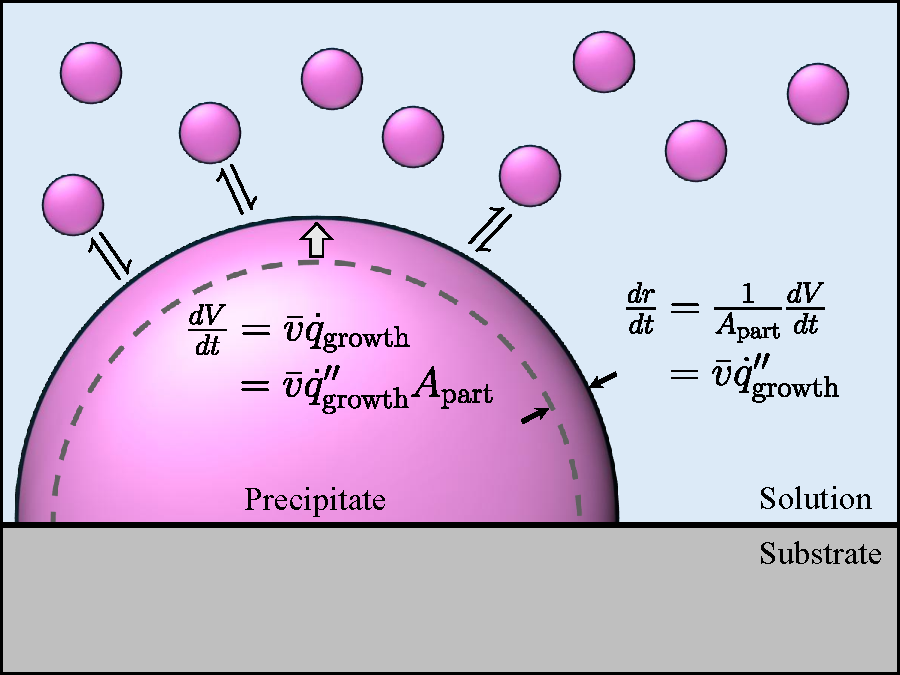
\includegraphics[scale=0.5]{figures/particle_growing_at_size.pdf} 
    \caption{Herein, we assume hemispherical particles and a constant molar deposition rate $\dot{q}_\mathrm{growth}^{\prime\prime}$. This results in a radial growth rate $\tfrac{dr}{dt}$ that does not depend on particle size, providing a simple means of evaluating the PSD tracking scheme's accuracy.}
    \label{fig:deposition}
\end{figure}

\subsection{Algorithms for PSD Tracking} % Describe the model and show results 
The model discretizes the PSD into uniform bins of fixed differential radius $\Delta r$. The following discussion focuses on particle growth, but the same principles apply to stripping reactions. Herein, we explore three separate PSD tracking algorithms:
\subsubsection{Algorithm 1: Simple finite differencing}
Our first approach uses finite differencing to track the number of particles entering and exiting each bin. All bins have the same thickness $\Delta r_{\mathrm{bin}}$, and the centroid of each bin represents a fixed radius.  Therefore, at any point in time the variable $N_i$ in the solution vector represents the number density of particles with radius between $\Delta r \times i$ and $\Delta r \times (i+1)$.  The model is defined by a set of ordinary differential equations describing the temporal evolution of $N_i$ for $0\leq i \leq n_{\rm bins}$, where $n_{\rm bins}$ is the total number of bins. 
The first bin's radius equals the nucleation radius: $r_\mathrm{nuc}$. 
\begin{equation}
    r_0 = r_\mathrm{nuc}=\frac{\Delta r_\mathrm{bin}}{2}
    \label{eq:r_0}
\end{equation}
Nucleation only occurs in bin 0. The nucleation rate $\dot{q}_\mathrm{nuc}''$, and the fraction of the total surface area $f_A$ available for deposition (i.e. that fraction not already blocked by deposits) determine the particle deposition rate in this bin (particles per m$^2$ per s). Once deposited, particles grow, leaving bin 0 and entering bins with larger average radii, once their radius exceeds the value $\Delta r$. 

When discretizing, particles are evenly spaced within a bin, meaning $x\%$ of the bin width contains $x\%$ of the $N_i$ particles in bin $i$. Fractional distance within a bin therefore equals the fraction of the  particles in the bin that occupy that distance. If the particle radii grow by one-quarter of the thickness of a bin during a timestep ($\frac{dr}{dt}\Delta t=0.25\Delta r_\mathrm{bin}$), then one-quarter of the particles in the bin should exit to the next bin, during that time step. The number of particles leaving a bin is therefore equal to the radial growth rate divided by the bin thickness, times the number density of particles in the bin. The differential equation for the number density of particles in bin $i=0$ is therefore:
\begin{equation}
     \frac{dN_0}{dt}=f_A\dot{q}_\mathrm{nuc}'' - \frac{\frac{dr}{dt}}{\Delta r_{\mathrm{bin}}}N_0,
     \label{eq:bin 0 sfd}
\end{equation}
where the fraction of available surface area $f_A = 1 - N_0 \pi r_{\rm nuc}^2$.  For bins with radii larger than $r_{\rm nuc}+\frac{\Delta r}{2}$, there is no nucleation, only growth.  Particles `enter' a bin by growing too large for the preceding smaller bin, and particles  `exit' by growing too large and entering the next largest bin. Entry and exit rates follow the logic laid out in eq.~\ref{eq:bin 0 sfd}. For a bin $i>0$, we therefore have: %The flux of particles outgrowing bin $i$ is equal and opposite to the flux of particles entering bin $i+1$. The same fraction of particles will be displaced from all intermediate bins as a consequence of uniform radial growth. 
\begin{equation} 
     \frac{dN_i}{dt}=\frac{\frac{dr}{dt}}{\Delta r_{\mathrm{bin}}}\left(N_{i-1} - N_{i}\right)
     \label{eq:bin i sfd}
\end{equation}
The total number of bins and the bin thickness therefore determine the average radius of the largest bin, $i=n_{\rm bins}$. 
\begin{equation}
    r_{\rm max} = \Delta r\times n_{\rm bins}
    \label{eq:r_max}
\end{equation}
No particles can exit this bin, leading to the following differential equation:
\begin{equation}
    \frac{dN_N}{dt}=\frac{\frac{dr}{dt}}{\Delta r_{\mathrm{bin}}}N_{n_{\rm bins}-1}
    \label{eq:bin N sfd}
\end{equation}
Consequently, the largest bin is not intended to contain an appreciable number of particles. If it does, that is a signal that more bins are needed for the simulation.

\begin{figure}[b!]
    \centering
    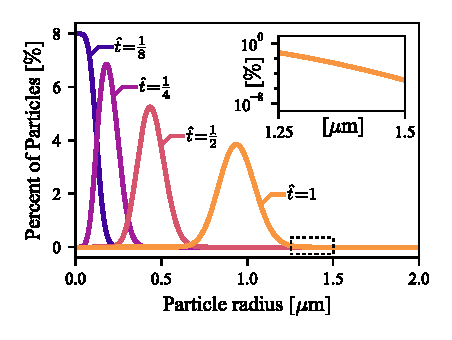
\includegraphics[scale=1]{figures/Plot with inset.pdf} 
    \caption{Simulated PSD snapshots using Algorithm 1: simple finite differencing. Non-dimensional time $\hat{t}$ is scaled by the total simulation time (4 s). The observed `flattening' of the PSD shape with time is inconsistent with the model assumptions, and the maximum radius far exceeds the theoretical maximum of 1 $\mu$m (see inset), revealing shortcomings in this model approach.}
    \label{fig:init_model}
\end{figure}
The simulation results for Algorithm 1 are shown in Figure \ref{fig:init_model}. The figure shows four PSD snapshots, each as a function of non-dimensional time $\hat{t}$, normalized by the total simulation time (4s). The nucleation rate is constant and stops at $\hat{t}=\frac{1}{8}$. Even though the growth rate is the same for all particles, regardless of radius, the PSD in Figure~\ref{fig:init_model} widens and flattens with time, indicating inconsistency with the underlying model assumptions. Particles prematurely exit the leading bin and linger in trailing bins. Moreover, while the constant growth rate $\frac{dr}{dt} = 0.25\, \mu$m s$^{-1}$ implies a maximum radius of 1 $\mu$m after the 4s-long simulation, we observe a significant population of particles with $r > 1 \,\mu$m and some small number of particles with $r > 1.5\,\mu$m (see inset).  Similarly, at the trailing edge, the last nuclei formed at $\hat{t} = \frac{1}{8}$ should have a radius of 0.875 $\mu$m at $\hat{t}=1$. Instead, Figure~\ref{fig:init_model} shows an appreciable portion of the PSD with $r \leq 0.75 \mu$m.

The errors of this algorithm are due to homogenization within the spatial mesh: for a bin $i$, the algorithm does not discriminate between particles that are barely larger than $r_i - \frac{\Delta r}{s}$ and those that are barely smaller than $r_i + \frac{\Delta r}{2}$. In any bin, entering particles should be required to grow by $\Delta r$ before they can exit. Instead, homogenization in algorithm 1 dictates that as soon as $N_i > 0$ for a bin $i$, a fraction of the particles can immediately grow out of the bin and into bin $i+1$. In the trailing bin, the only way all particles will leave a bin is if  growth during a time step, $\frac{dr}{dt}\Delta t$, exceeds $\Delta r$. Otherwise, some fraction of the particles will always remain, reminiscent of Zeno's paradox.

\subsubsection{Algorithm 2: `Bookmarking' the PSD upper and lower limits}
To enforce maximum and minimum radii consistent with the model assumptions, algorithm 2 includes leading and trailing ``bookmarks" that track the smallest and largest particle radii, respectively, as illustrated in Figure ~\ref{fig:BM_diagram}. The leading bookmark prevents particles from prematurely exiting the largest occupied bin and the trailing bookmark prevents particles from remaining too long in the trailing bin. Both bookmarks begin at $r_0$ and advance at the rate $\frac{dr}{dt}$. The leading bookmark moves immediately and the trailing bookmark moves once nucleation ceases (this last simplification is for easily interpretable results; other approaches can be implemented, if desired). 

Equations~\ref{eq:bin 0 sfd},~\ref{eq:bin i sfd}, and~\ref{eq:bin N sfd} apply to bins with no bookmarks at time $t$. Modifications are required for any bin with a bookmark. The leading bookmark regulates the particle flux leaving the largest occupied bin, referred to as the leading bin. When the leading bookmark moves within a bin, no particles leave the bin. Particles enter from the previous bin as they did in equation \ref{eq:bin i sfd}:
\begin{equation}
    \frac{dN_{i,lbm}}{dt}=\frac{\frac{dr}{dt}}{\Delta r_{\mathrm{bin}}}N_{i-1},
    \label{eq:bin i lbm stays}
\end{equation}
\begin{equation}
    \frac{dN_{i,lbm+1}}{dt}=0.
     \label{eq:bin i+1 lbm stays}
\end{equation}
where $i,lbm$ is the index of the leading bin. Equations \ref{eq:bin i lbm stays} and \ref{eq:bin i+1 lbm stays} prevent the runaway `forward diffusion' of particles observed in Figure~\ref{fig:init_model}. In Figure ~\ref{fig:BM_diagram}a, the vertical yellow line marks the location of the leading bookmark.\\

The bookmark position reflects the fact that particles do not occupy all radii equally within the leading bin. Only the portion of the leading bin behind the bookmark is occupied, and particles will not leave a bin until the leading bookmark advances to the next bin. When the leading bookmark advances to the next bin, the new leading bin is initially unoccupied. The transition from zero flux to finite flux in this bin leads to large residuals and small timestep when the bookmark crosses bin boundaries. The algorithm therefore approximates that a leading bookmark is always moving \emph{within} a bin. The error introduced by neglecting the number or particles that move between bins during the same time step as the bookmark is negligibly small.\\

The trailing bookmark guarantees that particles do not reside in the trailing bin for longer than the prescribed residence time, $\frac{\Delta r}{\frac{dr}{dt}}$. When the trailing bookmark moves within a bin, the fraction of particles that outgrow that bin equals the distance the radius grew in that timestep divided by the distance between the right edge of the bin and the bookmark at the start of the timestep:
\begin{equation}
    \frac{dN_i}{dt}=-\frac{\frac{dr}{dt}}{\Delta r_{\mathrm{bin}}-r_\mathrm{tbm}}N_{i}(t),
    \label{eq:bin i tbm stays}
\end{equation}
\begin{equation}
    \frac{dN_{i+1}}{dt}=\frac{\frac{dr}{dt}}{\Delta r_{\mathrm{bin}}-r_\mathrm{tbm}}N_{i}(t)-\frac{\frac{dr}{dt}}{\Delta r_{\mathrm{bin}}}N_{i+1}(t).
    \label{eq:bin i+1 tbm stays}
\end{equation}
When the trailing bookmark approaches a bin's edge, the denominator in equation~\ref{eq:bin i tbm stays} decreases, leading to smaller time steps. As with $r_{lbm}$, the algorithm approximates that the trailing bookmark always moves \emph{within} a bin.

\begin{figure}
    \centering
    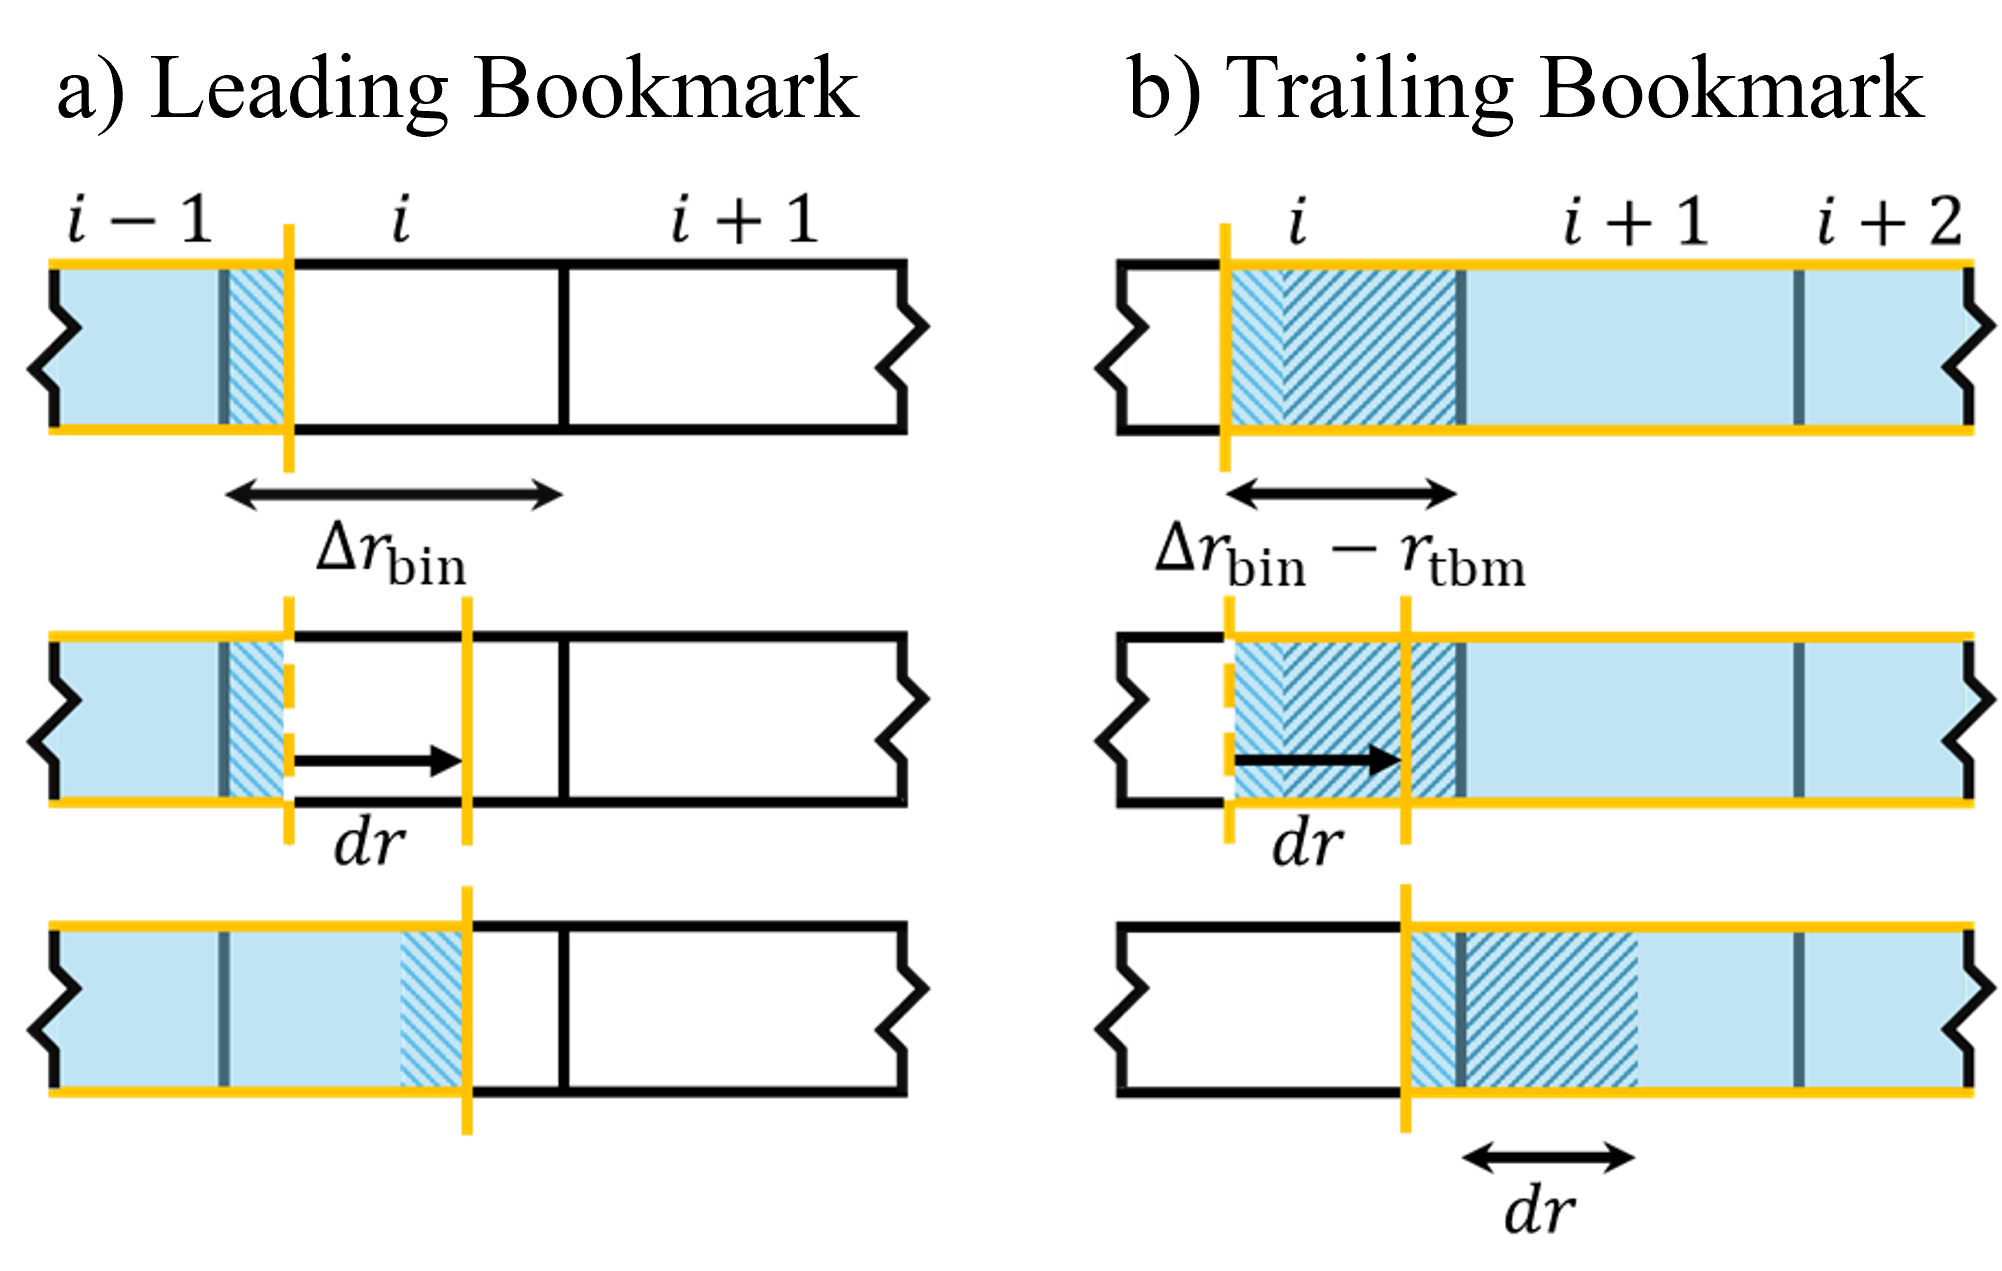
\includegraphics[scale=0.5]{figures/BM_combined.png}
    \caption{The bookmarks start and end in bin $i$. Each row depicts the same set of bins at different stages of a single timestep. The top is the initial state, the middle is the change, and the bottom is the final state. The bookmark moves at the radial growth rate and its progress in single timestep is $dr$. The patterned fill marks the portion of particles that begin the timestep in the bin with the bookmark. \textbf{a)} The leading bookmark  prevents particles from prematurely exiting the bin.
    \textbf{b)} The trailing bookmark controls the particle flux leaving the trailing bin. The fraction of particles that leave the trailing bin is equal to the darker patterned portion divided by the entire patterned portion.}
    \label{fig:BM_diagram}
\end{figure}

\begin{figure}[h]
    \centering
    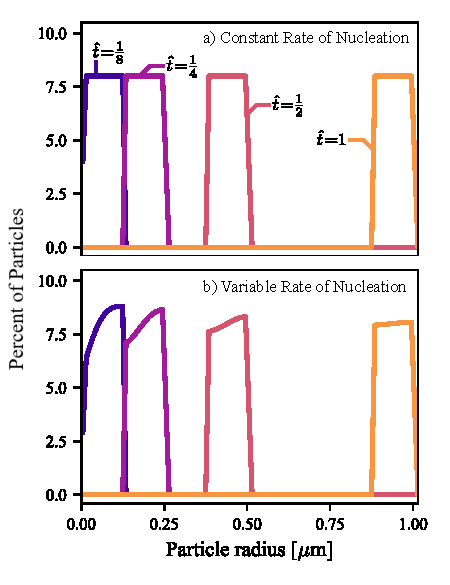
\includegraphics[scale=1]{figures/PSD_with_bms.pdf}
    \caption{ PSD snapshots during a simulation using Algorithm 2: `Bookmarks.'  \textbf{a)} Constant nucleation rate. Bookmarks halt the premature flux of particles shown in Figure ~\ref{fig:init_model}.
    \textbf{b)} Variable nucleation rate. Here, the bookmarks enforce the correct minimum and maximum radius. However, the PSD `flattening' from Figure~\ref{fig:init_model}, while contained by the bookmarks,  still occur between these limits.}
    \label{fig:PSD_BM}
\end{figure}
The simulation in Figure \ref{fig:PSD_BM}a uses the bookmark approach and a constant nucleation rate. Results show that the bookmarks successfully enforce growth limits at the leading and trailing edges of the PSD. However, the algorithm fails when the nucleation rate varies with time, as shown in Figure \ref{fig:PSD_BM}b. Both simulations have constant growth rates and stopped nucleating at $\hat{t} = \frac{1}{8}$. The profile widths in Figure ~\ref{fig:PSD_BM} are invariant with time. However, the PSD profile still changes with time in Figure ~\ref{fig:PSD_BM}b. As above, the flattening of the PSD within its bounds Figure~\ref{fig:PSD_BM}b stems from the assumption that particles are evenly distributed within bins. 

% ==================== Model 3: Moving Hopper ==================================
\subsubsection{Algorithm 3: The `moving hopper' model}
In our model, nucleation is the sole mechanism capable of establishing or altering the PSD shape; growth shifts the entire profile while maintaining constant relative spacing between particle sizes. One way to visualize the deposition process is as a hopper above a conveyor belt. The hopper is positioned at the start of the belt and the nucleation rate determines how many particles flow through the hopper into the bins below. As the particles grow, the conveyor belt moves the bins and their particles to new sizes, while new bins appear under the hopper to receive nuclei. This is visualized in Figure \ref{fig:Conveyorbel_Moving_Hopper}a, where bins move down the conveyor belt at the growth rate. The particle radius in the bin directly under the hopper is $r_\mathrm{nuc}$, and each subsequent bin's radius is calculated by adding $\Delta r_{\rm bin}$ to the radius of the previous bin. Translating this concept directly into code, while accurate, would require the number of state variables to vary dynamically. \\
\begin{figure*}
    \centering
    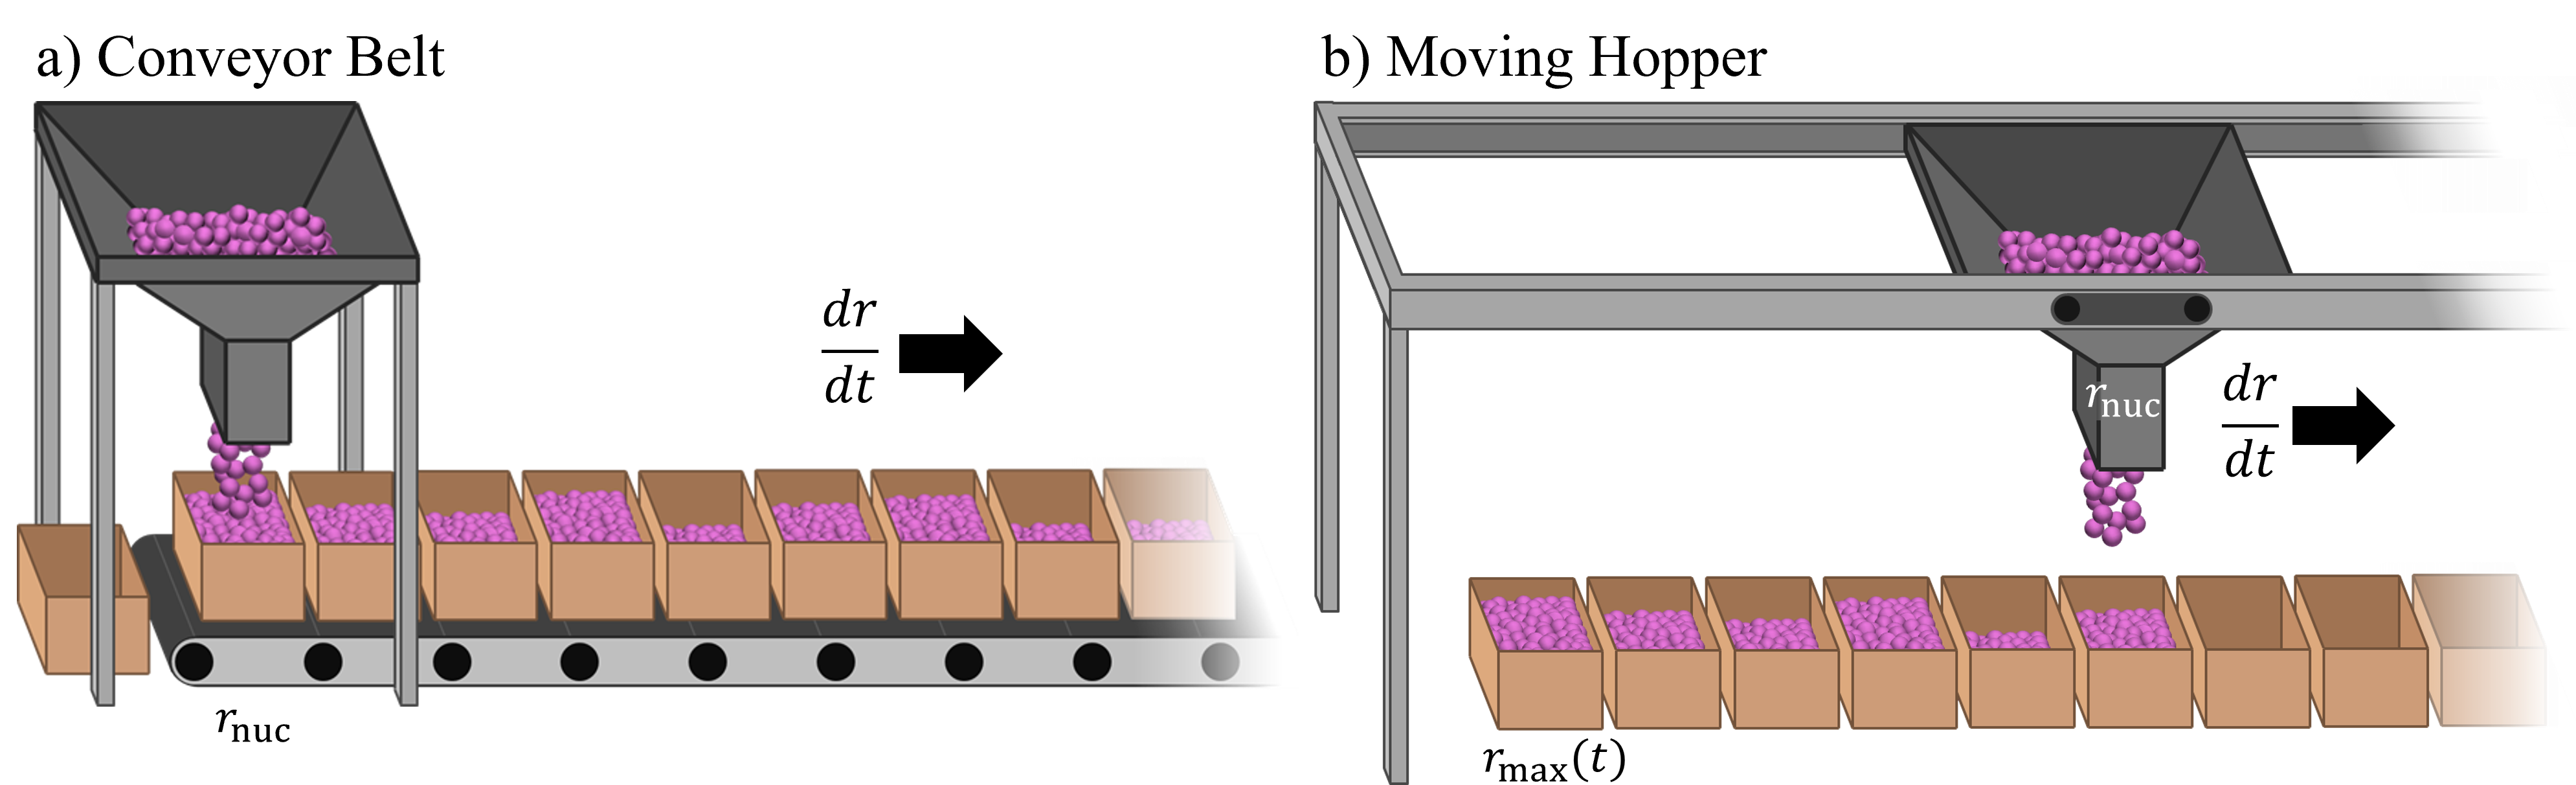
\includegraphics[scale=0.5]{figures/ConveyorBelt_MovingHopper_Horiz.png}
    \caption{\textbf{a)} A static hopper deposits particles while bins move on a semi-infinite conveyor belt below. All particles are deposited at the nucleation radius, and grow at the same rate, $\frac{dr}{dt}$. The radius of each bin changes as the particles grow.  \textbf{b)} The simulation is re-envisioned, where hopper moves along semi-infinite tracks above unmoving boxes. The foundational concepts are the same as in a), but this set up is easier to translate into code. The leftmost bin will always have the largest radius, and hopper always deposits particles at the nucleation radius.}
    \label{fig:Conveyorbel_Moving_Hopper}
\end{figure*}
 To avoid dynamically resizing the solution vector, our approach re-envisions the coordinate system such that the deposited particles do not move between bins. Rather, $r_i$, the average radius of particles in any bin $i$ changes with time; $N_i$, the number density of particles in bin $i$ only changes when $r_i = r_{\rm nuc}$.  Figure \ref{fig:Conveyorbel_Moving_Hopper}b illustrates the concept. The `hopper,' indicating the bin where $r_i = r_\mathrm{nuc}$, begins at $i = 0$ at $t_0$, and moves to the right ($i > 0$) at the growth rate $\frac{dr}{dt}$. The number of particles in a bin can only change if the hopper is located over that bin at time $t$ (note that the hopper can also remove particles due to stripping reactions; this is not implemented here, for simplicity). A local coordinate system moves with the hopper, defined by one additional variable: $r_0$ the radius of bin zero at time $t$, which also corresponds to the maximum radius. Because the growth rate does not vary with particle radius in this simulation, all other radii between $0 \leq r_i \leq r_0$ are determined as:
 \begin{equation}
     r_i = r_0 - i\times \Delta r_{\rm bin}
     \label{eq:ri_hopper}
 \end{equation}
Equation~\ref{eq:ri_hopper} is needed during post processing, but not during the simulation. The bin directly beneath the hopper at a given time is that with radius $0\leq r \leq r_\mathrm{nuc}+\frac{\Delta r_{\rm bin}}{2}$, determined via modulus division. This leads to the following set of differential equations:
        \begin{equation}
            \frac{dN_{i_{\rm nuc}}}{dt} = f_A\dot{q}^{\prime\prime}_{\rm nuc}\hspace{2em}{\rm For}\, i = i_{\rm nuc}
        \end{equation}
    
        \begin{equation}
            \frac{dN_{i}}{dt} = 0 \hspace{2em}{\rm For\, all\, other}\,i
        \end{equation}
        \begin{equation}
            \frac{dr_0}{dt} =\overline{v}_{\rm dep}\dot{q}^{\prime\prime}_{\rm growth}
        \end{equation}
where $\overline{v}_{\rm dep}$ is the molar volume of the deposited material.
\begin{figure}[h]
    \centering
    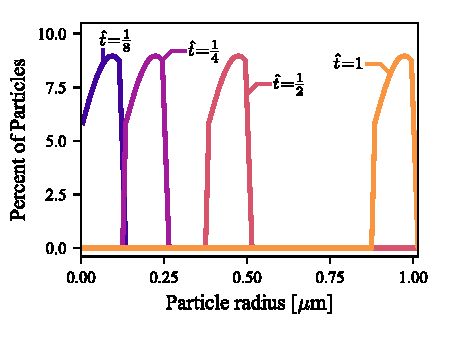
\includegraphics[scale=1]{figures/PSD_moving_hopper.pdf}
    \caption{Four snapshots of the PSD during a simulation using Algorithm 3 and a variable nucleation rate. The PSD is invariant, and moves at the radial growth rate.}
    \label{fig:PSD_cb}
\end{figure}
Figure~\ref{fig:PSD_cb} shows the results of this algorithm. The shape of the PSD in Figure~\ref{fig:PSD_cb} is invariant, consistent with the model assumptions, even when $\dot{q}^{\prime\prime}_{\rm nuc}$ varies with time. Moreover, the maximum radius at the simulation's end equals the predicted size. Unlike in Figure~\ref{fig:PSD_BM}b, there is no `flattening' of the PSD during the simulation, demonstrating a suitable approach for PSD tracking during HNG reactions.

\subsection{Discussion}
Initial attempts at tracking particle growth resulted in flattening between bins that distorted the PSD. The `moving hopper' model implemented here controls which bin particles are deposited into instead of moving particles between bins. It also only requires two differential equations, at any given time. The model implemented here assumes that particles deposit and grow as hemispheres with a uniform radial growth rate for all particles. However, the implications of our findings are relevant even if the radial growth rate is a function of radius, or the shapes of the particles are not uniform. Any finite differencing scheme that moves particles between discrete bins and assumes even particle distribution within bins will cause the PSD to flatten over time.  The algorithm here also provides a pathway for situations where $\dot{q}^{\prime\prime}_{\rm growth}$ \emph{does} vary with particle radius. In this situation, particles in bin $i$ are related not just by size, but also temporally: particles deposited at the same time will evolve in a uniform manner.  In this situation, tracking $N_i$ and $r_i$ for every bin will permit radially-dependent growth rates.

To support open science practices, the code for the three algorithms is publicly available on GitHub at \bluelink{https://github.com/t-koberna/LiS/tree/letter}{https://github.com/t-koberna/LiS/tree/letter}. \\ 


\section{Author Information}
Corresponding Author \\
\textbf{Steven C. DeCaluwe} - Department of Mechanical Engineering, Colorado School of Mines, Golden, Colorado 80401, United States; \bluelink{https://orcid.org/0000-0002-3356-8247}{\orcidlink{0000-0002-3356-8247}\,https://orcid.org/0000-0002-3356-8247} Email: \bluelink{decaluwe@mines.edu}{decaluwe@mines.edu}

Author\\
\textbf{Trent Koberna} - Department of Mechanical Engineering, Colorado School of Mines, Golden, Colorado 80401, United States \bluelink{https://orcid.org/0009-0004-0141-0535}{\orcidlink{0000-0002-3356-8247}\,https://orcid.org/0009-0004-0141-0535} 
\section{Acknowledgments}
This work was funded by the U.S. Department of Energy (DOE) grant EE0011168 from the Vehicle Technologies Office (program lead Simon Thompson).
% References
\bibliographystyle{unsrt}
\bibliography{bibliography}

\end{document}